\documentclass{article}

\usepackage{kafkanotes}

%Judul dan Penulis
\title{Tulis Judul Disini}
\author{Muhammad Gaffar A.A.}

\begin{document}

%Halaman Judul
\begin{titlepage}
\thispagestyle{empty}
\maketitle

%Abstrak
\begin{abstract}
(Style: Kafka-Notes v0.1, terinspirasi dari Style Tufte). Lorem ipsum dolor sit amet, consectetur adipiscing elit. Morbi luctus tristique justo, a ultricies nibh. Duis at diam vitae neque consequat pellentesque quis maximus mauris. Phasellus tempus sem a est accumsan, vel rhoncus urna rutrum. Nam pulvinar dignissim sapien feugiat consequat. Ut ac elit in velit facilisis gravida vel eu tortor. Praesent id finibus nisl, eget mattis ex. Pellentesque habitant morbi tristique senectus et netus et malesuada fames ac turpis egestas. Ut a orci a justo euismod pharetra. Pellentesque ornare tortor non dignissim ultrices. Etiam hendrerit scelerisque ex, in pellentesque dolor tincidunt id. Nunc sodales urna a enim maximus, at lacinia eros vulputate. Vestibulum non tempus ex, ac aliquam urna. Integer luctus ullamcorper felis aliquet varius. Sed mauris diam, accumsan vel porta vitae, pulvinar eget eros. Phasellus pretium felis eget sapien cursus, at accumsan lorem congue. Etiam egestas est non nisi tristique, id consequat tellus efficitur. 
\end{abstract}

\tableofcontents
\end{titlepage}

%Geometri untuk halaman konten
\newgeometry{top=20mm,bottom=25mm,right=80mm,left=20mm}

%================KONTEN DIMULAI DISINI================%

\section{Paragraf dan Persamaan Sederhana}
Lorem ipsum dolor sit amet, consectetur adipiscing elit. Aliquam viverra ante felis. Interdum et malesuada fames ac ante ipsum primis in faucibus. Vestibulum non fermentum erat. Pellentesque ut porta orci. Proin ultrices purus ex, vitae dictum sem laoreet nec. Aenean tempus, elit vitae eleifend lacinia, nunc orci porttitor mauris, a congue nisi turpis eu nisi. Donec non faucibus purus, nec pretium dui. Proin pretium vulputate sem, et aliquet leo varius eget. In ut tortor sed nibh aliquam luctus eu gravida purus. Aenean arcu urna, feugiat at viverra vel, tristique fringilla sem. Duis vestibulum dolor in neque varius eleifend. 
\begin{equation}
\mathcal{R}^{\text{d}} = g^e_{\sigma_{2}}\left(\frac{\Gamma^z}{Q_{12}^2-M_W^2}\right)
\end{equation}
Proin convallis interdum libero a sollicitudin. In dignissim quam id viverra congue. Pellentesque eget magna massa. Quisque sit amet sagittis felis. Proin a ipsum quis magna sodales egestas non euismod turpis. Sed nisi purus, vestibulum vitae volutpat auctor, euismod sit amet mauris. 

\begin{margintable}
\centering
\begin{tabular}{||c c c c||} 
 \hline
 Col1 & Col2 & Col2 & Col3 \\ [0.5ex] 
 \hline\hline
 1 & 6 & 87837 & 787 \\ 
 2 & 7 & 78 & 5415 \\
 3 & 545 & 778 & 7507 \\
 4 & 545 & 18744 & 7560 \\
 5 & 88 & 788 & 6344 \\ [1ex] 
 \hline
\end{tabular}
\captionsetup{justification=centering}
\caption{Table to test captions and labels}
\end{margintable}

Aenean neque mauris, consectetur luctus lacinia vel, viverra a magna. Donec rhoncus venenatis hendrerit.

\subsection{Subsection dan Tabel}
Lorem ipsum dolor sit amet, consectetur adipiscing elit. Proin sit amet augue sollicitudin, eleifend risus non, scelerisque elit. In tempus dictum nisl nec convallis. Fusce congue, lacus ut mattis lacinia, nulla dolor ultricies sem, eu molestie velit quam et felis. Fusce mattis, dolor vel cursus egestas, tortor nibh efficitur tortor, eget venenatis velit orci ut est. Praesent a diam leo. Vestibulum consectetur vel augue sit amet facilisis. Etiam vitae lorem ut lectus tincidunt feugiat. Interdum et malesuada fames ac ante ipsum primis in faucibus. Nullam sem nulla, posuere sed felis ut, porttitor sagittis lorem. Nam lacus mi, laoreet non fringilla a, eleifend eget turpis. Maecenas ultricies aliquam felis. 

Lorem ipsum dolor sit amet, consectetur adipiscing elit. Proin sit amet augue sollicitudin, eleifend risus non, scelerisque elit. In tempus dictum nisl nec convallis. Fusce congue, lacus ut mattis lacinia, nulla dolor ultricies sem, eu molestie velit quam et felis. Fusce mattis, dolor vel cursus egestas, tortor nibh efficitur tortor, eget venenatis velit orci ut est. Praesent a diam leo. Vestibulum consectetur vel augue sit amet facilisis. Etiam vitae lorem ut lectus tincidunt feugiat. Interdum et malesuada fames ac ante ipsum primis in faucibus. Nullam sem nulla, posuere sed felis ut, porttitor sagittis lorem. Nam lacus mi, laoreet non fringilla a, eleifend eget turpis. Maecenas ultricies aliquam felis. 

\subsection{Sidenote dan Gambar}

\begin{marginfigure}%
  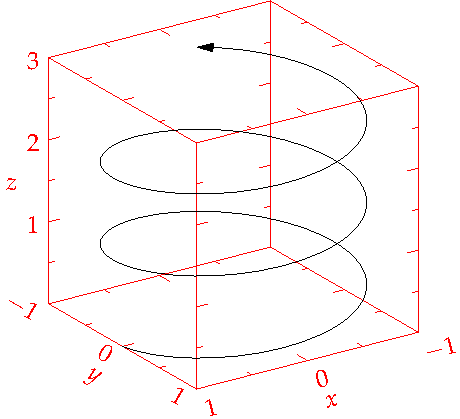
\includegraphics[width=\linewidth]{gambar/helix}
  \caption{This is a margin figure.  The helix is defined by 
    $x = \cos(2\pi z)$, $y = \sin(2\pi z)$, and $z = [0, 2.7]$.  The figure was
    drawn using Asymptote (\url{http://asymptote.sf.net/}).}
  \label{fig:marginfig}
\end{marginfigure}

In hac habitasse platea dictumst. Sed elementum pellentesque justo at ultricies. Nunc dapibus nisl nec massa sollicitudin commodo. Nulla sagittis neque ex, in dictum tellus ultricies ut. Integer vulputate metus id ligula efficitur rutrum. Etiam ut est et neque feugiat egestas. Integer ac lacinia urna. 
Nullam enim nisl, venenatis at luctus malesuada, ultricies rutrum tortor. Aliquam ut nulla congue, pharetra magna vitae, sollicitudin mi. Vestibulum mattis imperdiet sapien ac ornare. In id sagittis sem. Nunc luctus ex sit amet eros posuere viverra. Praesent tristique arcu sed urna rhoncus, vitae aliquam libero mollis. Proin condimentum purus congue arcu mattis sodales. Suspendisse ullamcorper vulputate egestas. Mauris placerat venenatis urna in feugiat. Morbi dignissim arcu nunc. Cras imperdiet neque neque, vel posuere lorem elementum at. 
In hac habitasse platea dictumst. Sed elementum pellentesque justo at ultricies. Nunc dapibus nisl nec massa sollicitudin commodo. Nulla sagittis neque ex, in dictum tellus ultricies ut. Integer vulputate metus id ligula efficitur rutrum.
Nullam enim nisl, venenatis at luctus malesuada, ultricies rutrum tortor. Aliquam ut nulla congue, pharetra magna vitae, sollicitudin mi. Vestibulum mattis imperdiet sapien ac ornare. In id sagittis sem. Nunc luctus ex sit amet eros posuere viverra
In hac habitasse platea dictumst. Sed elementum pellentesque justo at ultricies. Nunc dapibus nisl nec massa sollicitudin commodo. Nulla sagittis neque ex, in dictum tellus ultricies ut. Integer vulputate metus id ligula efficitur rutrum. Etiam ut est et neque feugiat egestas. Integer ac lacinia urna. 
Nullam enim nisl, venenatis at luctus malesuada\sidenote{Ini adalah contoh sidenote yang baik dan benar. Sidenote dapat digunakan untuk catatan tambahan, ataupun referensi.}, ultricies rutrum tortor. Aliquam ut nulla congue, pharetra magna vitae, sollicitudin mi. Vestibulum mattis imperdiet sapien ac ornare. In id sagittis sem. Nunc luctus ex sit amet eros posuere viverra.

\section{Persamaan panjang}
Phasellus congue gravida venenatis. Phasellus blandit, nisi et sagittis luctus, turpis quam ultricies mauris, a sollicitudin nulla eros non velit. Proin pellentesque tortor lacus, sed vehicula leo congue vel. Cras molestie dolor lacus, ut posuere quam sagittis sit amet. Nulla dapibus vehicula massa et pulvinar. Donec consectetur mauris sit amet consequat rhoncus. Donec finibus dapibus consequat. Praesent nec imperdiet metus. Suspendisse nec consectetur ex, eu cursus metus. Maecenas a justo sit amet elit dapibus suscipit. Nulla facilisi. Suspendisse iaculis vulputate risus. 
Disarankan untuk tidak memakai nomor persamaan pada persamaan yang panjang.
\begin{equation}
W = \frac{1}{2\mu_0}\left[\frac{\Psi'^2 \pi^2}{b^2} \sum_{m,n} a_{mn}^2 n^2 (ab/4) + \frac{\Psi'^2 \pi^2}{a^2} \sum_{m,n} a_{mn}^2 m^2 (ab/4) + \Psi'^2ab\left(\mu^2 + \sum_{m,n} \frac{8a_{mn} \mu^2}{\pi^2 mn} + \frac{a_{mn}^2 \mu^2}{4}\right)\right]\notag
\end{equation}

\subsection{Gambar dengan Lebar Lebih Besar}
In sed eros non purus lacinia fermentum nec eget ligula. Praesent viverra varius ligula, quis cursus mi porttitor nec. Pellentesque vitae lobortis orci. Nullam eu iaculis libero. Pellentesque habitant morbi tristique senectus et netus et malesuada fames ac turpis egestas. Praesent finibus accumsan urna quis vestibulum. Ut vel ipsum non magna egestas faucibus non faucibus odio. Vestibulum convallis tincidunt velit. Integer non vestibulum magna. Nunc et urna non magna dictum luctus sed a purus. Fusce pharetra commodo enim, sit amet fermentum mauris tempus vitae. 
Taruh gambar dalam kolom paragraf, namun caption taruh di margin kanan.

\begin{figure*}[!h]\centering
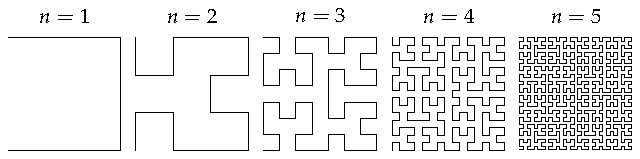
\includegraphics[scale = 1.08]{gambar/hilbertcurves}
\caption{\footnotesize A caption with long text bla bla bla bla
  bla bla bla bla bla bla bla bla bla bla bla bla bla bla}
\end{figure*}

\end{document}